\documentclass[11pt,a4paper,fleqn, onesside]{article}
%
\usepackage[T1]{fontenc}
\usepackage{amsmath, amssymb, amsthm}
\usepackage[danish,english]{babel}

\usepackage[ansinew]{inputenc}
%\usepackage[utf8]{inputenc} %Der skal anvendes utf8
\usepackage{epsfig}
\usepackage{graphicx}
\usepackage[]{mcode}
\usepackage{lmodern}
\usepackage{float}
\usepackage{setspace}
\usepackage{lscape}
\usepackage{hyperref}
\usepackage{cleveref}
\crefname{equation}{}{equations}
\crefname{figure}{figure}{figures}
\usepackage{tabu}
\usepackage{graphicx}
\usepackage{caption}
\usepackage{multirow}
\usepackage{spverbatim}
\onehalfspacing

\usepackage[top=25mm, left=30mm, right=30mm,bottom=25mm,headsep=10mm, footskip=12mm]{geometry}
%
\usepackage{fancyhdr}
\pagestyle{fancyplain}
\lhead[\thepage]{}

\begin{document}

\begin{titlepage}
\begin{center}
\vspace{4cm}
\Huge{\sc 31310 Linear Control Design 2}\\
\vspace{0.8cm}
\large{\sc Compulsory Assignment 2015 : Loudspeaker control\\}
\vspace{1.2cm}
%\Huge {\sc Exam Report}\\
%\vspace{2cm}
\normalsize{by}\\
\vspace{1.2cm}
{\sc
\large Katleen Blanchet s150798  \\ 
Titouan Boulmier s150810\\
}
%\o{}
\vspace{2cm}
\begin{center}
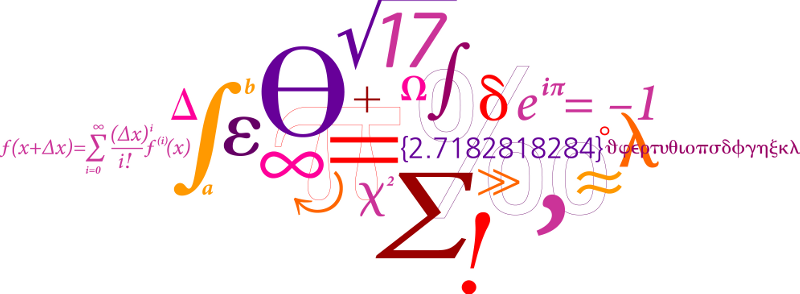
\includegraphics[scale=2.2]{dtulogo2.jpg}
\end{center} 
\vspace{3.1cm}
\normalsize{\today}\\
\vspace{1.37cm}
\includegraphics[scale=0.7]{dtulogo.jpg}\\
\vspace{0.2cm}
\normalsize{Technical University of Denmark \\ Department of Electrical Engineering \\
}
\end{center}
\end{titlepage}
%\newpage
\thispagestyle{empty}
\selectlanguage{english}

\pagebreak
\pagenumbering{Roman}
\setcounter{page}{1}
\setcounter{tocdepth}{4}
\setcounter{secnumdepth}{4} 
\tableofcontents
\newpage
\pagenumbering{arabic}


\part{Exercise 1: Distortion Attenuation for Loudspeakers}
\chapter{Moving-coil Loudspeakers}
\section{Loudspeakers electrical equivalent circuit}

\begin{figure}[H]
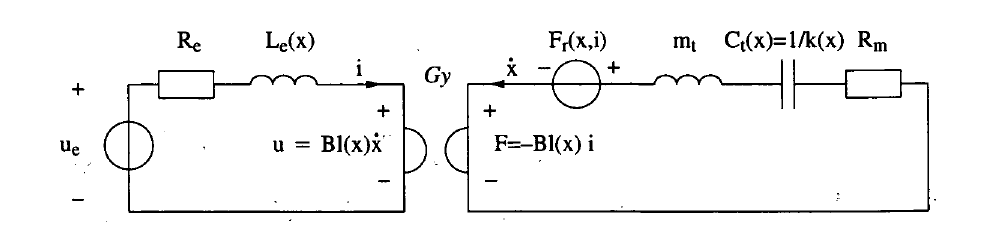
\includegraphics[scale=.6]{figures/circuit.png}
\caption{Electrical equivalent lumped element model of the voltage driven electrodynamic loudspeaker for low frequencies. The coupling between the
electrical and mechanical domain is performed through the gyrator with gy-
ration constant Bl(x).}
\label{circuit}
\end{figure}

\begin{align} 
  u_e &= R_ei+\frac{dL_e(x)}{dx}\frac{dx}{dt}i+L_e(x)\frac{di}{dt}+Bl(x)\frac{dx}{dt} \label{eq:1.1} \\     
  Bl(x)i &= m_t\frac{d^2x}{dt^2}+R_m\frac{dx}{dt}+k(x)x-\frac{1}{2}\frac{dL_e(e)}{dx}i^2 \label{eq:1.2}
\end{align}
where
\begin{align}
  Bl(x) &= Bl_0+b_1x+b_2x^2 \label{eq:1.3}  \\
  L_e(x) &= L_{e0}+l_1x+l_2x^2 \label{eq:1.4}  \\
  k(x) &= k_0+k_1x+k_2x^2 \label{eq:1.5} 
\end{align}

\subsection{Problem 1}
By means of Eqs~\ref{eq:1.1},~\ref{eq:1.2},~\ref{eq:1.3},~\ref{eq:1.4} and~\ref{eq:1.5}, we can identify 3 state variables $x$,  $\dot{x}$ and $i$. We can also identify the input $u_e$.

$\text{x}=\begin{pmatrix}
   x \\
   \dot{x} \\
	 i
\end{pmatrix}$ and $\text{u}=(u_e)$

Then, we can derive the nonlinear dynamical state space model to obtain

\begin{align}
   \dot{x} &= \dot{x}\\
	 \ddot{x} &= \frac{(Bl_0+b_1x+b_2x^2)i-R_m\dot{x}-(k_0+k_1x+k_2x^2)x+\frac{1}{2}(l_1+2l_2x)\dot{x}i^2}{m_t}\\
	 \dot{i} &= \frac{u_e-(R_e+(l_1+2l_2x)\dot{x}^2)i-(Bl_0+b_1x+b_2x^2)\dot{x}}{L_{e0}+l_1x+l_2x^2}
\end{align}

In matrix format, we have

\begin{equation}
	\label{eq:eqModel}
	\dot{\text{x}}=f(\text{x})+g(\text{x})\text{u}
\end{equation}
with
\begin{equation}
	\label{eq:f(x)}
	f(\text{x})=\begin{pmatrix}
   \text{x}(2) \\
	 \frac{(Bl_0+b_1\text{x}(1)+b_2\text{x}(1)^2)\text{x}(3)-R_m\text{x}(2)-(k_0+k_1\text{x}(1)+k_2\text{x}(1)^2)\text{x}(1)+\frac{1}{2}(l_1+2l_2\text{x}(1))\text{x}(2)\text{x}(3)^2}{m_t}\\
	 \frac{-(R_e+(l_1+2l_2\text{x}(1))\text{x}(2)^2)\text{x}(3)-(Bl_0+b_1\text{x}(1)+b_2\text{x}(1)^2)\text{x}(2)}{L_{e0}+l_1\text{x}(1)+l_2\text{x}(1)^2}
\end{pmatrix}
\end{equation}
\begin{equation}
	\label{eq:g(u)}
	g(\text{x})=\begin{pmatrix}
   0\\
   0 \\
	 1
\end{pmatrix}
\end{equation}

\subsection{Problem 2}
The block diagram of the nonlinear model figure \ref{fig:figP2} in Appendix \ref{AppP2} shows how the electrical and the mechanical subsystems are interconnected. This block diagram is also our SIMULINK model. The system is quickly stabilised (around 1 s) but as we are going to analyse it in the frequency domain, a longer period of time will provide better results. Thus, the TIME\_SIM is set to 5 s. 


  \begin{thebibliography}{2}

  \end{thebibliography}

\end{document}
